\documentclass[12pt]{article}

\usepackage{fouriernc}
\usepackage{amssymb}
\usepackage{amsmath}
\usepackage{amsfonts}
\usepackage[utf8]{inputenc}
\usepackage[T1]{fontenc}
\usepackage[margin=1in]{geometry}
\usepackage{graphicx}

\graphicspath{ {./images/} }

\newcommand{\curly}[1]{\left\{      #1 \right\}     }
\newcommand{\round}[1]{\left(       #1 \right)      }
\newcommand{\hard} [1]{\left[       #1 \right]      }
\newcommand{\abs}  [1]{\left|       #1 \right|      }
\newcommand{\floor}[1]{\left\lfloor #1 \right\rfloor}
\newcommand{\ceil} [1]{\left\lceil  #1 \right\rceil }

\setlength{\parindent}{0in}

\title{Homework 2}
\author{Tim Harding}

\begin{document}
\maketitle

\section*{1.3.4.a}

\subsection*{Problem}
Negate the following statement:

$\forall B \in \mathbb{R}$, $\exists A \in \mathbb{R}, A \geq a$ such that $\forall x > A \implies f(x) > B$.

\subsection*{Solution}
$\exists B \in \mathbb{R}$, $\forall A \in \mathbb{R}, A \geq a$ such that $\exists x > A \implies f(x) \leq B$.



\section*{1.3.4.b}

\subsection*{Problem}
Negate the following statement:

$\forall B \in \mathbb{R}$, $\exists A \in \mathbb{R}, A \geq a$ such that $\forall x > A \implies f(x) < B$.

\subsection*{Solution}
$\exists B \in \mathbb{R}$, $\forall A \in \mathbb{R}, A \geq a$ such that $\exists x > A \implies f(x) \geq B$.



-- TODO --
\section*{1.3.6}

\subsection*{Problem}
Show that the following statement is false:
\begin{align*}
    \lim_{x \to \infty} \cos(x) = 0
\end{align*}

\subsection*{Proof}
Positive:
For all $\epsilon > 0$, there exists $x_0 = $ such that when $x > x_0$ we have $\abs{\cos(x) - 0} \leq 1 < \epsilon$.

$\forall \epsilon > 0, \exists x_0 = a : \forall x > x_0 \implies \abs{\cos(x) - 0} \leq 1 < \epsilon$

There exists $\epsilon_0 = $ such that for all $x$,

$\exists \epsilon_0 = arst, \forall x, \exists x_0 = arst > x \implies \abs{\cos(x_0) - 0} \geq 0$



\section*{2.1.8}

\subsection*{Problem}

Negate the following definition:

$\forall \epsilon > 0,\ \exists \delta \in (0, \delta_0],\ \forall x : 0 < \abs{x - x_0} < \delta \implies \abs{f(x) - L} < \epsilon$.

\subsection*{Solution}
$\exists \epsilon > 0,\ \forall \delta \in (0, \delta_0],\ \exists x : 0 < \abs{x - x_0} < \delta \implies \abs{f(x) - L} > \epsilon$.



\section*{2.1.10.a}

\subsection*{Problem}
Given $\epsilon = 0.314$, find $\delta$ such that $\forall x : \abs{x} < \delta \implies \abs{(4x + 7) - 7} < \epsilon$.

\subsection*{Solution}
\begin{align*}
    \abs{4x} &< \epsilon \\
    \abs{x} &< \frac{\epsilon}{4}
\end{align*}
We require $\delta = \frac{0.314}{4} = \boxed{0.0785}$.



\section*{2.1.10.b}

\subsection*{Problem}
Find another $\tilde{\delta} \neq \delta$ that works.

\subsection*{Solution}
Any smaller choice of $\delta$ will work, such as $\boxed{0.05}$.



\section*{2.1.10.c}

\subsection*{Problem}
What is the greatest satisfactory choice of $\delta$?

\subsection*{Solution}
The solution from part a is the largest possible choice of $\delta$, $\boxed{0.0785}$.



\section*{2.1.12}

\subsection*{Problem}
Find $L$ such that
\begin{align*}
    \lim_{x \to -2} \round{x^2 - 2x + 4} = L
\end{align*}
and prove it.

\subsection*{Solution}
The limit is $L = (-2)^2 - 2(-2) + 4 = 4 + 4 + 4 = 12$. For proof,

$\forall \epsilon > 0,\ \exists \delta = \min(\frac{\epsilon}{7}, 1),\ \forall x : 0 < \abs{x - (-2)} < \delta \implies \\ \abs{(x^2 - 2x + 4) - 12} = \abs{x^2 - 2x - 8} = \abs{x + 2} \abs{x - 4} \leq 7 \abs{x - (-2)} < \epsilon$.



\section*{2.1.15.a}

\subsection*{Problem}
Given $f(x) = \frac{1}{x}$, find all $x_0$ such that $\lim_{x \to x_0} f(x)$ exists.

\subsection*{Solution}
$\frac{1}{x}$ has one jump discontinuity at $x = 0$, so $x_0 \in \curly{r \in \mathbb{R} : r \neq 0}$.



\section*{2.1.15.b}

\subsection*{Problem}
Find all $x_0$ such that $f(x)$ is continuous at $x_0$.

\subsection*{Solution}
$f(x)$ is continuous where the limit and $f(x_0)$ both exist and are equal, which is again true when $x_0 \in \curly{r \in \mathbb{R} : r \neq 0}$.



\section*{2.1.15.c}

\subsection*{Problem}
Prove parts (a) and (b)



\section*{2.1.16}

\subsection*{Problem}
Prove that
\begin{align*}
    \lim_{x \to 1} \frac{x}{x + 1} &= \frac{1}{2}
\end{align*}

\subsection*{Solution}
$\forall \epsilon > 0, \exists \delta = \min\round{\frac{3}{2}, \epsilon}$ st $\forall x : 0 < \abs{x - 1} < \delta \implies \abs{\frac{1}{x + 1} - \frac{1}{2}} = \abs{\frac{2 - (x + 1)}{2(x + 1)}} = \abs{\frac{-x + 1}{2(x + 1)}} = \abs{x - 1} \frac{1}{2} \abs{\frac{1}{x + 1}} < \abs{x - 1} < \epsilon$



\section*{2.1.18}

\subsection*{Problem}
Prove that $\sqrt{x}$ is continuous on $(0, \infty)$.

\subsection*{Solution}
\begin{enumerate}
    \item Trivially, $\sqrt{x}$ exists for all inputs in the range $(0, \infty)$.
    \item We now show that the limit $\lim_{x \to a} \sqrt{x}$ exists for all $a$ in $(0, \infty)$. $\forall \epsilon,\ \exists \delta = arst : 0 < \abs{x - a} < \delta \implies \abs{\sqrt{x} - \sqrt{a}} < \epsilon$
\end{enumerate}



\section*{2.2.6.a}

\subsection*{Problem}
Given
\begin{align*}
    f(x) = \begin{cases}
        4x + 7 & x < 1 \\
        -2x + 12.99 & x \geq 1
    \end{cases}
\end{align*}
Graph the function.

\subsection*{Solution}
\begin{center}
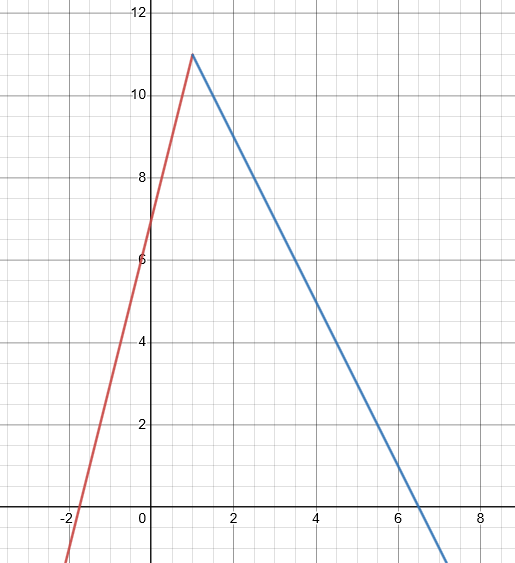
\includegraphics[width=8cm]{2.2.6}
\end{center}



\section*{2.2.6.b}

\subsection*{Problem}
Find the two one-sided limits

\begin{enumerate}
    \item To show that $\lim_{x \to 1^{-}} f(x) = 11$, we show that $\forall \epsilon > 0,\ \exists \delta = \min\round{1,\ \frac{\epsilon}{4}},\ \forall x : 0 < 1 - x < \delta \implies \abs{4x + 7 - 11} = \abs{4x - 4} = 4\abs{x - 1} = 4 \abs{1 - x} < \epsilon$.
    \item To show that $\lim_{x \to 1^{+}} f(x) = 10.99$, we show that $\forall \epsilon > 0,\ \exists \delta = \min\round{1,\ \frac{\epsilon}{2}},\ \forall x : 0 < x - 1 < \delta \implies \abs{2x + 12.99 - 10.99} = \abs{2x - 2} = 2\abs{x - 1} < \epsilon$.
\end{enumerate}



\section*{2.2.6.c}

\subsection*{Problem}
What can be said about $\lim_{x \to 1} f(x)$?

\subsection*{Solution}
The limit does not exist because $\lim_{x \to 1^-} f(x) \neq \lim_{x \to 1^+} f(x)$.



\section{2.2.6.d}

\subsection*{Problem}
Does the limit exist at $x = 0$, $x = 1$, or $x = 2$?

\subsection*{Solution}
We have shown that because of the discontinuity, the function is not continuous at $x = 1$. However, there is no discontinuity at $x = 0$ or $x = 2$ and the limit is equal to the function evaluated at each of these points, so the function is continuous in those places.



\section*{2.2.8}

\subsection*{Problem}
Prove that
\begin{align*}
    \lim_{x \to 0^-} \frac{\abs{x}}{x} = -1
\end{align*}

\subsection*{Solution}
$\forall \epsilon > 0, \exists \delta = 1, \forall x : 0 < 0 - x < \delta \implies \abs{\frac{\abs{x}}{x} - (-1)} = \abs{\frac{-x}{x} + 1} = \abs{-1 + 1} = 0 < \epsilon$.



\section*{2.2.9}

\subsection*{Problem}
Find all values of $x$ for which $\lim_{x \to 0^-} \frac{\abs{x}}{x} = \lim_{x \to 0^+} \frac{\abs{x}}{x}$ using rigorous methods.

\subsection*{Solution}




\section*{2.2.10}

\subsection*{Problem}
Show that
\begin{align*}
    \lim_{x \to 0^+} \round{x + \sqrt{x}} = 0
\end{align*}

\subsection*{Solution}
$\forall \epsilon > 0,\ \exists \delta = \frac{\epsilon}{2},\ \forall x : 0 < x - 0 < \delta \implies \abs{x + \sqrt{x} - 0} < \abs{2x} = 2x < \epsilon$.

\section*{2.3.5}

\subsection*{Problem}
Rewrite the original and negation of definition 2.3.1 using quantifiers.

\subsection*{Solution}
\begin{enumerate}
    \item $\forall M,\ \exists \delta \in (0, \delta_0],\ \forall x : 0 < \abs{x - x_0} < \delta \implies f(x) > M$.
    \item $\exists M,\ \forall \delta \in (0, \delta_0],\ \exists x : 0 < \abs{x - x_0} < \delta \implies f(x) \leq M$.
\end{enumerate}



\section*{2.3.6}

\subsection*{Problem}
Rewrite the original and negation of question 2.3.2 using quantifiers.
\begin{align*}
    \lim_{x \to x_0} f(x) &= -\infty \\
    \lim_{x \to x_0^+} f(x) &= \pm\infty \\
    \lim_{x \to x_0^-} f(x) &= \pm\infty \\
\end{align*}

\subsection*{Solution}
Originals:
\begin{enumerate}
    \item $\forall M < 0, \exists \delta, \forall x : 0 < \abs{x - x_0} < \delta \implies f(x) < M$
    \item $\forall M < 0, \exists \delta, \forall x : 0 < x - x_0 < \delta \implies f(x) < M$
    \item $\forall M > 0, \exists \delta, \forall x : 0 < x - x_0 < \delta \implies f(x) > M$
    \item $\forall M < 0, \exists \delta, \forall x : 0 < x_0 - x < \delta \implies f(x) < M$
    \item $\forall M > 0, \exists \delta, \forall x : 0 < x_0 - x < \delta \implies f(x) > M$
\end{enumerate}

Negations:
\begin{enumerate}
    \item $\exists M < 0, \forall \delta, \exists x : 0 < \abs{x - x_0} < \delta \implies f(x) \geq M$
    \item $\exists M < 0, \forall \delta, \exists x : 0 < x - x_0 < \delta \implies f(x) \geq M$
    \item $\exists M > 0, \forall \delta, \exists x : 0 < x - x_0 < \delta \implies f(x) \leq M$
    \item $\exists M < 0, \forall \delta, \exists x : 0 < x_0 - x < \delta \implies f(x) \geq M$
    \item $\exists M > 0, \forall \delta, \exists x : 0 < x_0 - x < \delta \implies f(x) \leq M$
\end{enumerate}



\section*{2.3.9}

\subsection*{Problem}
Show that
\begin{align*}
    \lim_{x \to 0^-} \frac{1}{x} = -\infty
\end{align*}

\subsection*{Solution}
$\forall M < 0, \exists \delta = \frac{1}{M}, \forall x : 0 < 0 - x < \delta \implies \frac{1}{x} < M$



\section*{2.3.10}

\subsection*{Problem}
Show that
\begin{align*}
    \lim_{x \to 1} \frac{1}{(x - 1)^2} = \infty
\end{align*}

\subsection*{Solution}
$\forall M > 0,\ \exists \delta = \frac{1}{\sqrt{M}} + 1,\ \forall x : 0 < \abs{x - 1} < \delta \implies \frac{1}{(x - 1)^2} > M$



\section*{2.3.11}

\subsection*{Problem}
Show that
\begin{align*}
    \lim_{x \to 0^+} \frac{x - 1}{x^2} = -\infty
\end{align*}

\subsection*{Solution}
$\forall M < 0,\ \exists \delta = M,\ \forall x : 0 < x - 0 < \delta \implies \frac{x - 1}{x^2} < x - 1 < x < M$


\end{document}
